\chapter{Implementation}
\label{chap:implementation}

This chapter discusses the implementation of a proof of concept concretizing the specification introduced in \Cref{chap:analysis-design}.

The language of choice was Scala, primarily for the following reasons:
%
\begin{itemize}
    \item its advanced features (e.g. mixins, family polymorphism, higher kinded types, and so on) and flexible syntax make it a really powerful language to express DSLs (Domain Specific Languages) with a few lines of code;
    \item Scala 3's new features, in particular \textit{context functions} and \textit{extension methods}, allow for an even more concise syntax;
    \item ScaFi could be used as a guide throughout the development process, so it was possible to mimic its internal structure using similar constructs offered by the language.
\end{itemize}

\section{Architecture}
\label{sec:architecture}

The project is structured into layers following the diagram shown in \Cref{fig:architecture}.
%
\begin{figure}
    \centering
    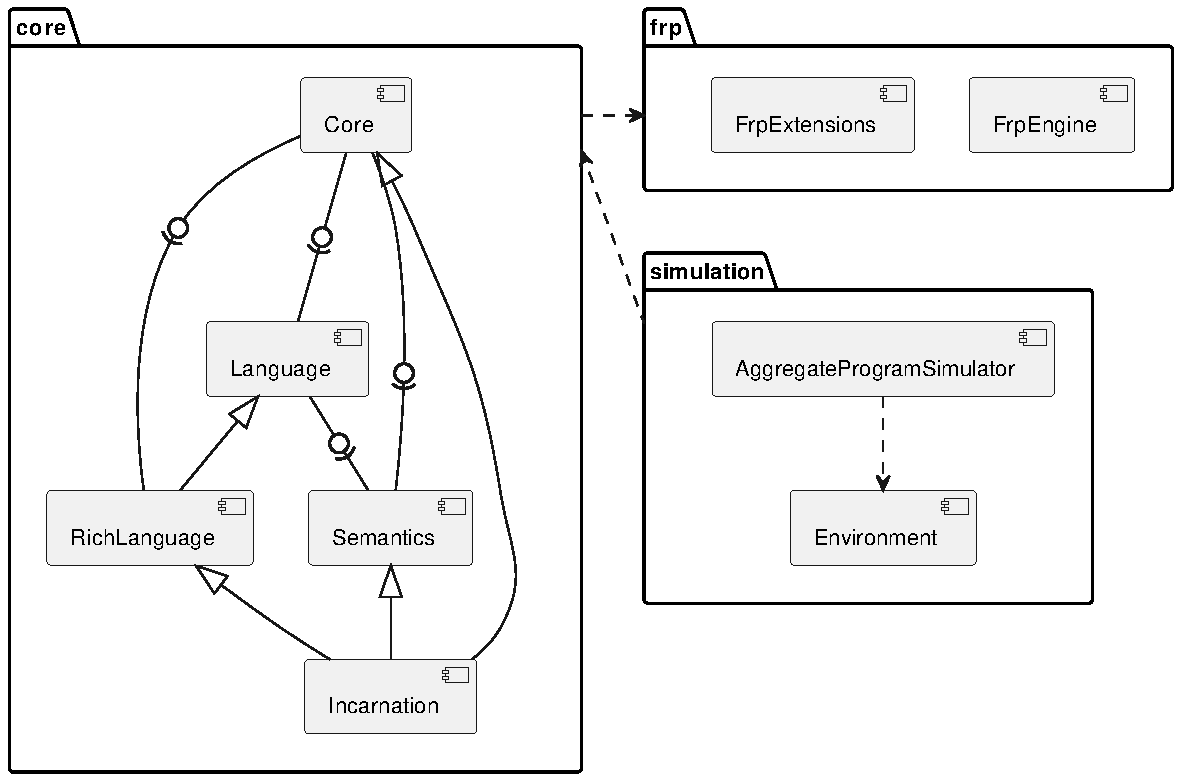
\includegraphics[width=\textwidth]{figures/diagrams/architecture.pdf}
    \caption{High level architecture, corresponding in part to the package structure.}
    \label{fig:architecture}
\end{figure}
%
Their responsibilities can be summarized as follows:
%
\begin{itemize}
    \item the \textbf{FRP} layer is the one exposing the FRP engine (as described in \Cref{sec:frp}, using the Sodium library), also adding some extensions on top of that;
    \item the \textbf{Core} layer is the beating heart of the library, modeling and implementing the specification of \Cref{sec:specification};
    \item the \textbf{Simulation} layer provides a basic simulator capable of running aggregate programs for a network of devices.
\end{itemize}

Each layer, along with its sub-components, is described in greater detail in the sections below.

\section{FRP layer}

The FRP layer deals with cells and streams in order to provide expressive building blocks to the \textit{core} layer.
%
As stated before, this layer was implemented by leveraging the Sodium library and adding some extension methods and utilities to be used while defining the behavior of the aggregate constructs.

Some of these extensions include:
%
\begin{itemize}
    \item \textit{calming}, that is, a way to create a cell whose listeners are only notified of an update if the previous value is different from the new one, for performance reasons;
    \item \textit{buffering}, which refers to a mechanism by which events of a stream are collected for a certain amount of time before being emitted all at once, using some combination of the events that were buffered;
    \item \textit{throttling}, a particular way of buffering which combines element of the buffer by returning the last one that was received.
\end{itemize}

% TODO: show snippets of throttling and/or calming.

\section{Core layer}

The core layer follows an organization that is highly inspired to the core of ScaFi.
%
In fact, it models the entire specification as being broken down into \textit{components}, each providing a narrow set of features that can be combined together.
%
A way to model component-based structures using Scala is through \textit{mixins} and \textit{self-types}, which were used extensively during the development of the core layer.
%
These features, along with Scala's \textit{abstract type members}, enable the use of \textit{family polymorphism} \cite{10.1007/3-540-45337-7_17} to model complex domains.
%
In particular, the structure of the model presented in the specification was re-adapted in order to fit in the idiomatic practices of Scala and to be implemented via family polymorphism.
%
This guarantees a greater flexibility when introducing changes to the specification and allows extensions of the language to be introduced with little or no work at all.

\subsection{Core}

The root of the domain is given by the \texttt{Core} trait (\Cref{lst:core}).
%
\lstinputlisting[
	float,
	language=scala,
	caption={The \texttt{Core} trait, the root of the family polymorphism.},
	label={lst:core},
]{listings/Core.scala}
%
It defines the main concepts of an aggregate computation, namely:
%
\begin{itemize}
    \item an abstract \texttt{Context} type, since the specific way to interact with the environment is unknown at this point;
    \item an abstract \texttt{Export[+\_]} type, representing the output of a device with a \texttt{covariant} root type;
    \item an abstract \texttt{Path} type, denoting paths that can be looked up inside an \texttt{Export};
    \item the \texttt{Flow[A]} trait, defined in terms of the abstract types above in a way that is almost identical to the one defined in the specification, with the only difference being that the \texttt{Context} is passed implicitly.
\end{itemize}
%
This is the minimum required information that is used to perform an aggregate computation.

\subsection{Language}

Below \texttt{Core}, the \texttt{Language} trait introduces the constructs when mixed in with a \texttt{Core} object, from which the basic abstract types of aggregate computing are imported.
%
This is done via self-types, to avoid creating a strong inheritance hierarchy.
%
The \texttt{Language} trait is shown in \Cref{lst:language}
%
\lstinputlisting[
	float,
	language=scala,
	caption={The \texttt{Language} trait, introducing the main API of aggregate computing.},
	label={lst:language},
]{listings/Language.scala}
%
It introduces new abstract types that are specific to the constructs, in particular:
%
\begin{itemize}
    \item \texttt{DeviceId} denotes an identifier for devices participating in the aggregate computation;
    \item \texttt{LocalSensorId} and \texttt{NeighborSensorId} identify sensors that can be queried locally or from any neighbor, respectively;
    \item \texttt{NeighborField[+\_]} represents a mapping from DeviceIds to neighboring values of the given type.
\end{itemize}

A notable difference in how the language supports lifting operations (recall \Cref{sec:constructs-semantics}) is the fact that it is supported via a \textit{type class} and \textit{ad-hoc polymorphism}.
%
This was done by defining a \texttt{Liftable[F[\_]]} trait defining that a wrapper type \texttt{F[\_]}, generic in the type it encloses, supports lifting operations.
%
As stated before, lifting is a way for a function operating on atomic values to be applied to wrapped versions of those values, and this can be generalized to any function regardless of the number of parameters.
%
\texttt{Liftable[F[\_]]} supports lifting for functions that take up to three parameters.
%
However, lifting a unary function is more often \texttt{map}, and it is idiomatically more familiar when called as a method of the wrapper to be mapped, rather than as a top-level function.
%
This is why \texttt{map} is defined as an extension method while the binary and ternary versions are not.

The next lines of the \texttt{Language} trait declare the constructs of the language, maintaining the same API as defined by the specification.
%
In addition, since \texttt{NeighborField} is declared as an abstract type without any bounds, the language includes some of the operations that are needed, in particular by the \texttt{RichLanguage} trait.
%
In fact, \texttt{RichLanguage} introduces utilities that are built on top of the main API, which are primarily common folding operations on flows of neighbor fields, like \texttt{min} or \texttt{toSet}.

\subsection{Semantics}

The \texttt{Semantics} trait starts reifying the concepts that are defined by the \texttt{Core} and by the \texttt{Language}, giving an implementation of the constructs that corresponds to the one proposed in \Cref{sec:constructs-semantics}.
%
A portion of this trait can be found in \Cref{lst:semantics}, where some of the abstract types that were still unbound up to this point get reified, in particular:
%
\begin{itemize}
    \item \texttt{NeighborField[+A]} is reified as a \texttt{Map} from \texttt{DeviceId}s (still unbound at this stage) to \texttt{A}s;
    \item \texttt{Export[+A]} and \texttt{Path} are reified respectively as an \texttt{ExportTree[A]} and as a \texttt{Seq[Slot]}, for which the implementation is also included in the listing;
    \item \texttt{Context} gets bound to be a subclass of \texttt{BasicContext}, a new trait defined inside \texttt{Semantics}.
\end{itemize}
%
In addition, \texttt{Semantics} introduces a new abstract type \texttt{NeighborState} that is bounded to be a subclass of \texttt{BasicNeighborState}.
%
This way of dealing with \texttt{Context} and \texttt{NeighborState}, i.e. by only giving upper bounds, allows for greater flexibility and type safety when implementing classes inheriting from \texttt{Semantics}, while still enforcing some constraints that are needed at this abstraction level.
%
\lstinputlisting[
	float,
	language=scala,
	caption={A portion of the \texttt{Semantics} trait reifying some of the domain's abstract types.},
	label={lst:semantics},
]{listings/Semantics.scala}

The alignment process is implemented in the \texttt{alignWithNeighbors} method, shown in \Cref{lst:alignment}.
%
In practice, this corresponds to the construction of a cell holding maps that hold a certain value of type \texttt{T} for all neighbors aligned at a given path.
%
Each value \texttt{T} is extracted using a function \texttt{f} that take the current \texttt{NeighborState} and the sub-export at which the alignment happened with that neighbor.
%
Operationally, \texttt{alignWithNeighbors} deals with this concern by mapping the cell of the \texttt{NeighborStates} to a new one that constantly filters out neighbors that are not aligned by using the \texttt{followPath} method.
%
\lstinputlisting[
	float,
	language=scala,
	caption={Implementation of the alignment process.},
	label={lst:alignment},
]{listings/Alignment.scala}

As an example of the usage of \texttt{alignWithNeighbors}, the implementation of the \texttt{nbr} construct is presented in \Cref{lst:nbr}, which gathers the neighboring values located at \texttt{path + Nbr}, where \texttt{path} is the location where the \texttt{nbr} is being evaluated.
%
Subsequently, it replaces the old value computed at the previous evaluation with the new one exported by \texttt{a} before wrapping everything in a new export, following the semantics of \texttt{nbr}.
%
\lstinputlisting[
	float,
	language=scala,
	caption={Implementation of the \texttt{nbr} construct.},
	label={lst:nbr},
]{listings/Nbr.scala}

\subsection{Incarnation}

An \texttt{Incarnation} represents the final concretion in the core layer, defining a unified composition of all the traits that have been described up until this point.
%
Conceptually, it is a way to abstract away the details of a particular platform that is able to host an aggregate computation.
%
Practically, this is done by providing a \texttt{factory} that creates instances of the \texttt{Context} given some device identifier.
%
Its code is shown in \Cref{lst:incarnation}.
%
\lstinputlisting[
	float,
	language=scala,
	caption={The \texttt{Incarnation} trait.},
	label={lst:incarnation},
]{listings/Incarnation.scala}

Note that, even at this level, some of the abstract types defined by \texttt{Language} are not bound to any type yet, in particular \texttt{DeviceId}, \texttt{LocalSensorId} and \texttt{NeighborSensorId}.
%
The nature of those types is in fact platform specific, thus it is up to the specific implementation of \texttt{Incarnation} to decide what those should be concretely.

\section{Simulation layer}

This layer introduces a way to test the behavior of an aggregate program by running it in a simulated environment.
%
A simulation can in fact be carried out by creating \textit{in-memory} versions of the \texttt{Incarnation} and the \texttt{Context}, using synthesized data to replace sensors.

\subsection{Simulation incarnation}

The incarnation implemented for the testing purposes of this thesis is based on a certain network topology defined by an \texttt{Environment} object.
%
Simply put, an environment determines the number, the position and the neighboring relation of a device network in 2D space, assuming device identifiers are progressive integers.
%
\Cref{lst:environment} displays the definition of the trait modeling an \texttt{Environment}.
%
\lstinputlisting[
	float,
	language=scala,
	caption={The \texttt{Environment} trait.},
	label={lst:environment},
]{listings/Environment.scala}
%
The presence of an environment in the incarnation can be specified through a mixin, named \texttt{IncarnationWithEnvironment} (\Cref{lst:incarnation-with-environment})
%
\lstinputlisting[
	float,
	language=scala,
	caption={The \texttt{IncarnationWithEnvironment} mixin.},
	label={lst:incarnation-with-environment},
]{listings/IncarnationWithEnvironment.scala}
%
In addition, to favor modularity of the features of an incarnation, the simulation layer contains another pair of mixins that fix the bounds to the \texttt{LocalSensorId} and \texttt{NeighborSensorId} types for testing.
%
These mixins are respectively called \texttt{TestLocalSensors} and \texttt{TestNeighborSensors} (\Cref{lst:test-sensors}).
%
\lstinputlisting[
	float,
	language=scala,
	caption={The \texttt{TestLocalSensors} and \texttt{TestNeighborSensors} mixins.},
	label={lst:test-sensors},
]{listings/TestSensors.scala}

Finally, all mixins that have been described so far were combined together in order to create a concrete \texttt{Incarnation} to be used in the simulator, called \texttt{SimulationIncarnation} and presented in \Cref{lst:simulation-incarnation}.
%
\lstinputlisting[
	float,
	language=scala,
	caption={The \texttt{SimulationIncarnation} class.},
	label={lst:simulation-incarnation},
]{listings/SimulationIncarnation.scala}
%
The most relevant part of this incarnation in order to understand the \texttt{Simulator}, presented in \Cref{sec:simulator}, is the definition of the \texttt{SimulationContext}, specifically the implementation strategy of the \texttt{neighbors} method.
%
Internally, the context uses a wrapper of Sodium's \texttt{CellSink} (i.e. \texttt{IncrementalCellSink}) that is able to perform incremental updates by applying a function to the current state.
%
This is used to apply incremental updates to the state of neighbors as exports are received during program execution.
%
By calling \texttt{receiveExport} when a new export is received from one of the neighbors of the device, the context can be informed of a new neighbor state that can be registered in the sink, triggering all computations that depend on that state.

\subsection{Simulator}
\label{sec:simulator}

The final step towards simulating an aggregate computation is the simulator itself.
%
The phases of a simulation can be summarized as follows:
%
\begin{enumerate}
	\item \textbf{spawn contexts}: for each device participating in the computation, create a \texttt{Context} instance via the incarnation;
	\item \textbf{run the flow}: run the \texttt{Flow} that is being simulated on all the context instances, producing a cell of \texttt{Export}s for each device;
	\item \textbf{listen to export updates}: upon changes of any cell that was produced, broadcast that export to all the contexts of neighboring devices.
\end{enumerate}

\Cref{lst:simulator} shows the implementation of the \texttt{Simulator} class.
%
Its constructor takes as inputs an instance of \texttt{SimulationIncarnation}, that will be used to spawn context and to access the types defined by the model, and an optional \texttt{ExecutorService}, that is instead used to schedule notifications of export emissions in the background.
%
This is useful for performance and concurrency reasons, but most importantly it is required since Sodium does not allow listeners to call \texttt{send()} on \texttt{CellSink}s (which is called internally by the \texttt{receiveExport} method).
%
By scheduling these tasks on another control flow, this does not pose an issue.
%
\lstinputlisting[
	float,
	language=scala,
	caption={The \texttt{Simulator} class.},
	label={lst:simulator},
]{listings/Simulator.scala}

Notice that steps 2 and 3 are wrapped inside a transaction.
%
Other than guaranteeing that no \quotes{first events} are missed, wrapping both steps ensures that all flows start at the same logical instant, in a consistent fashion.
